\newpage
\section{Durchführung}
\label{sec:Durchführung}
\subsection{Aufbau}
\label{sec:aufbau}
Zu Beginn des Versuchs wird der optische Aufbau eingestellt, dazu müssen verschiedene optische Elemente 
ausgerichtet werden.
Der Aufbau ist schematisch in Abbildung \ref{fig:aufbau} dargestellt. Das von der Rubidium-Dampflampe
erzeugte Licht wird mit einer Linse zunächst kollimiert. Mit Hilfe eines Filters das $\text{D}_1$-Licht
transmittiert und der Rest abgeschirmt sortiert. Danach wird das Licht mit Hilfe eines Polarisationfilters
linear-polarisiert und anschließend mit einem $\sfrac{\symup{\lambda}}{4}$-Plättchen rechtszirkular-polarisiert.
Nach dem Hindurchtreten durch den Rubidiumdampf wird das Licht durch eine Sammellinse auf die Photozelle
fokussiert. Das Signal wird linear verstärkt und anschließend auf den Kanal 2 des Oszilloskops gegeben.

Des Weiteren befinden sich im Aufbau drei Helmholtz-Spulenpaare, zwei davon für das Horizontalfeld und eine für das Vertikalfeld.
Die Spulen für das Horizontalfeld teilen sich in eine Sweep-Spule mit einem Radius von $R=\SI{16.39}{\centi\meter}$ und
$N=\num{11}$ Wicklungen, sowie der Horizontalfeldspule mit einer Windungszahl von $N=\num{154}$ und einem 
Radius von $R=\SI{15.79}{\centi\meter}$ auf. Die Vertikalfeld-Spule besitzt $N=\num{20}$ Windungen, 
sowie den Radius $R=\SI{11.735}{\centi\meter}$. Jedes Spulenpaar besitzt seine eigene Stromquelle, dabei kann die Stromquelle der
Sweep-Spule linear durchgefahren werden.
Neben diesen Spulenpaaren gibt es noch ein Spulenpaar für das Hochfrequenzfeld, welches durch einen externen Frequenzgenerator
bereitgestellt wird.

\subsection{Kompensation des Erdmagnetfeldes}
\label{sec:erdmagnetfeld}
Bevor die Messung beginnen kann werden die beiden Linsen so positioniert in ihrer Höhe und Abständen, dass das Signal der Photozelle
maximal wird. Anschließend werden die drei anderen optischen Elemente eingesetzt, sodass der Strahl sie mittig passiert. Dabei werden
die Parameter der Verstärkung auf \num{1} gesetzt und die Zeitkonstante auf \SI{100}{\milli\second}. Ist alles eingestellt und optimiert,
so wird der Aufbau mit der schwarzen Decke abgedeckt.

Da die verwendeten Magnetfelder in dem Bereich der Erdmagnetfelder liegen, müssen diese zunächst kompensiert werden. Dazu wird der 
Strom durch die Spulen auf Null gedreht. Für die Sweep-Spule wird der 'Range' auf Maximum gestellt, ebenso wie 'Start' auf Minimum,
die Schalter auf 'Continuous' sowie 'Start' und die Periode auf \SI{2}{\second} gesetzt. Das Ausgangssignal der Sweep-Spule wird auf den 
Kanal 1 des Oszilloskops gegeben, dabei wird das Oszilloskop im XY-Betrieb betrieben. Für die Verstärkung der Photozelle wird 
'Gain' auf \num{20} gesetzt, 'Gain Multiplier' auf x\num{10} und 'Meter multiplier' auf x\num{2}.
Zunächst wird das Signal am Oszilloskop beobachtet, hier sollte ein Peak ähnlich zu dem in Abbildung \ref{fig:resonanz} links dargestellt 
sein. Dieser wird so schmal wie möglich gemacht, indem durch drehen des Tisches und den Strom durch die Vertikalspule (eine Umdrehung
entspricht \SI{0.1}{\ampere}) das Erdmagnetfeld kompensiert wird. Dazu kann sich an einem Kompass orientiert werden.

\subsection{Resonanz}
\label{sec:resonanz}
Um nun die Abstände der Zeeman-Niveaus auszumessen wird die sinusförmige Hochfrequenz im Wertebereich von \SIrange{100}{1000}{\kilo\hertz} 
mit $V_\text{PP} = \SI{4}{\volt}$ in \SI{100}{\kilo\hertz}-Schritten variiert.
Dabei wird die Position der auftretenden Peaks in Abhängigkeit vom Magnetfeld detektiert. Dazu wird der Schalter auf 'Reset' gestellt 
und das Magnetfeld verfahren bis zu dem Punkt an dem die Peaks ihr Minimum haben. Dabei entspricht eine Umdrehung gleich \SI{0.1}{\ampere}.
Für höhere Frequenzen wird zusätzlich zum Sweep-Feld auch das zweite Horizontalfeld eingesetzt, hier entspricht eine Umdrehung 
\SI{0.3}{\ampere}.

\begin{figure}
  \centering
  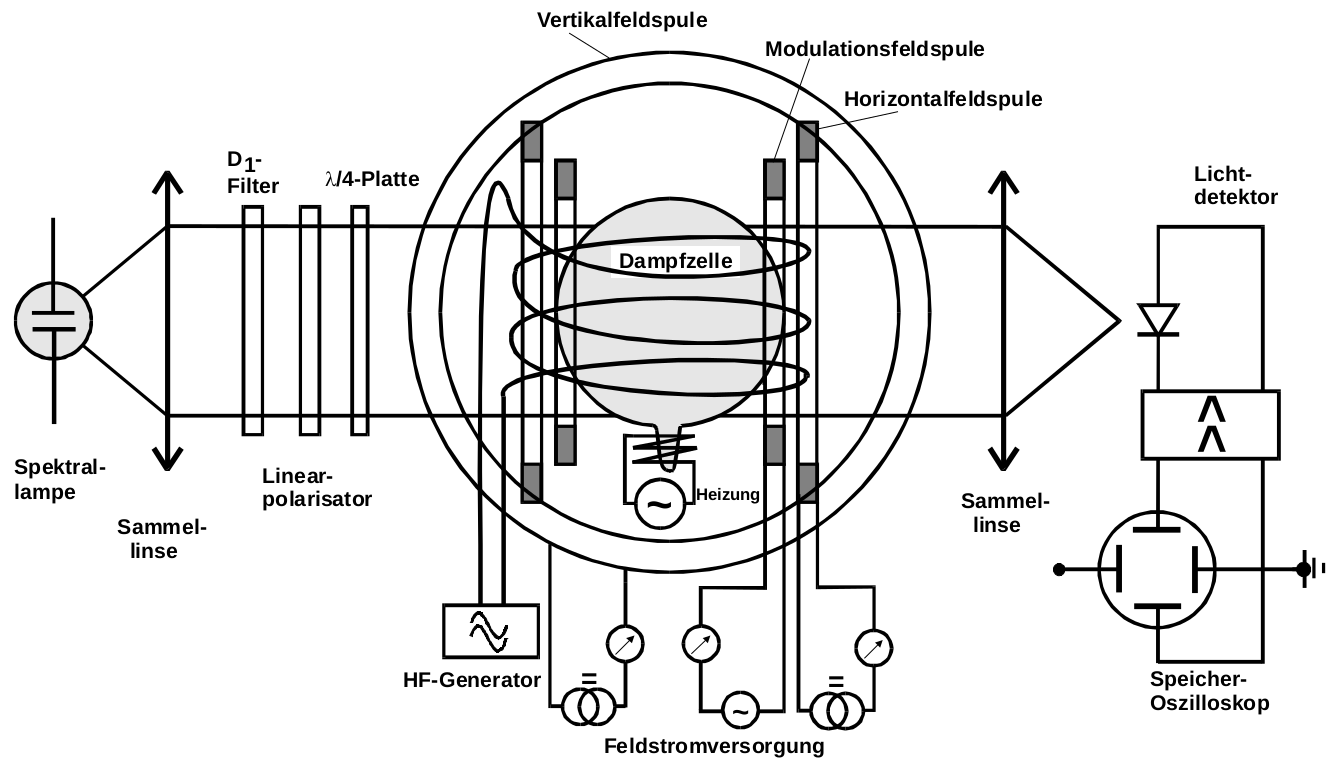
\includegraphics[height=8.0cm]{content/pictures/Aufbau.png}
  \caption{Schematische Darstellung des verwendeten Versuchsaufbaus \cite{anleitung}.}
  \label{fig:aufbau}
\end{figure}

\FloatBarrier